\pdfbookmark{Общая характеристика работы}{characteristic}             % Закладка pdf
\section*{Общая характеристика работы}

\newcommand{\actuality}{\pdfbookmark[1]{Актуальность}{actuality}\underline{\textbf{\actualityTXT}}}
\newcommand{\progress}{\pdfbookmark[1]{Разработанность темы}{progress}\underline{\textbf{\progressTXT}}}
\newcommand{\aim}{\pdfbookmark[1]{Цели}{aim}\underline{{\textbf\aimTXT}}}
\newcommand{\tasks}{\pdfbookmark[1]{Задачи}{tasks}\underline{\textbf{\tasksTXT}}}
\newcommand{\object}{\pdfbookmark[1]{Объект исследования}{object}\underline{\textbf{\objectTXT}}}
\newcommand{\subject}{\pdfbookmark[1]{Предмет исследования}{subject}\underline{\textbf{\subjectTXT}}}
\newcommand{\aimtasks}{\pdfbookmark[1]{Цели и задачи}{aimtasks}\aimtasksTXT}
\newcommand{\novelty}{\pdfbookmark[1]{Научная новизна}{novelty}\underline{\textbf{\noveltyTXT}}}
\newcommand{\influence}{\pdfbookmark[1]{Практическая значимость}{influence}\underline{\textbf{\influenceTXT}}}
\newcommand{\methods}{\pdfbookmark[1]{Методология и методы исследования}{methods}\underline{\textbf{\methodsTXT}}}
\newcommand{\defpositions}{\pdfbookmark[1]{Положения, выносимые на защиту}{defpositions}\underline{\textbf{\defpositionsTXT}}}
\newcommand{\reliability}{\pdfbookmark[1]{Достоверность}{reliability}\underline{\textbf{\reliabilityTXT}}}
\newcommand{\probation}{\pdfbookmark[1]{Апробация}{probation}\underline{\textbf{\probationTXT}}}
\newcommand{\contribution}{\pdfbookmark[1]{Личный вклад}{contribution}\underline{\textbf{\contributionTXT}}}
\newcommand{\publications}{\pdfbookmark[1]{Публикации}{publications}\underline{\textbf{\publicationsTXT}}}

\input{common/characteristic} % Характеристика работы по структуре во введении и в автореферате не отличается (ГОСТ Р 7.0.11, пункты 5.3.1 и 9.2.1), потому её загружаем из одного и того же внешнего файла, предварительно задав форму выделения некоторым параметрам

%Диссертационная работа была выполнена при поддержке грантов \dots

%\underline{\textbf{Объем и структура работы.}} Диссертация состоит из~введения,
%четырех глав, заключения и~приложения. Полный объем диссертации
%\textbf{ХХХ}~страниц текста с~\textbf{ХХ}~рисунками и~5~таблицами. Список
%литературы содержит \textbf{ХХX}~наименование.

\pdfbookmark{Содержание работы}{description}                          % Закладка pdf
\section*{Содержание работы}
Во \underline{\textbf{введении}} обосновывается актуальность
исследований, проводимых в~рамках данной диссертационной работы,
приводится обзор научной литературы по~изучаемой проблеме,
формулируется цель, ставятся задачи работы, излагается научная новизна
и практическая значимость представляемой работы.


\underline{\textbf{Первая глава}} посвящена краткому обзору подходов к
моделированию работы радиолокатора в режиме синтезирования апертуры.
В \textbf{подразделе 1.1} описываются энергетические, временные, частотные и
геометрические соотношения необходимость учёта которых составляет задачу
моделирования.
В \textbf{подразделе 1.2} описываются аналитические и точные методы для расчёта
электромагнитных полей.
В \textbf{подразделе 1.3} описываются приближенные методы для расчёта рассеянного поля
и эффективной поверхности рассеяния в частности.
Приведены особенности отдельных методов, существенные
для темы исследования диссертации.


\underline{\textbf{Вторая глава}} посвящена описанию использованных методов
расчёта рассеянного поля, которые позволяют производить эффективные
вычисления для сцен больш\'их электрических размеров.
В \textbf{подразделе 2.1} описаны принципы эффективной трассировки лучей.

Ускорение процесса трассировки лучей осуществляется через разбиение
пространства сцены в некоторую древовидную структуру. Два различных
подхода предполагают:
\begin{enumerate}
    \item
    K-мерные деревья;
    \item
    иерархии граничных объемов -- Bounding Vertex Hierarchy (BVH).
\end{enumerate}

Различие между двумя подходами заключается в принципе разделения сцены:
K-d деревья разделяют непосредственно сам объем, тем самым в структуре
дерева могут быть пустые листья. BVH задает граничный объем для объектов
на сцене, в свою очередь не позволяя создавать пустые листья в дереве.
Соответственно изменяются процедуры вставки и удаления элементов на
сцену, прохода по всему дереву и поиска ближайших соседей. Различия
между техниками представлены на рисунке~\ref{fig:octotree} и рисунке~\ref{fig:bvh}.

\begin{figure}[h]
    \centering
    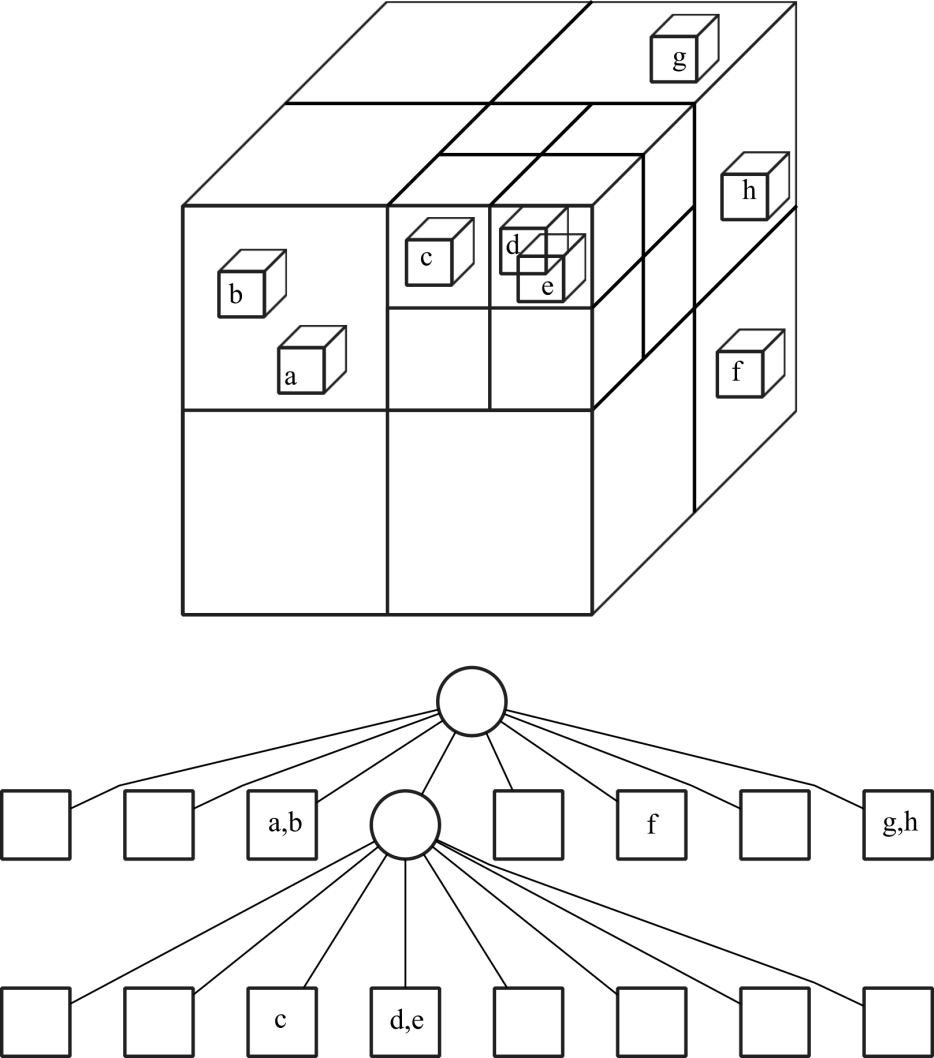
\includegraphics[width=0.5\linewidth]{Synopsis/images/octotree.png}
    \caption{Октодерево (К=3)}
    \label{fig:octotree}
\end{figure}


\begin{figure}[h]
    \centering
    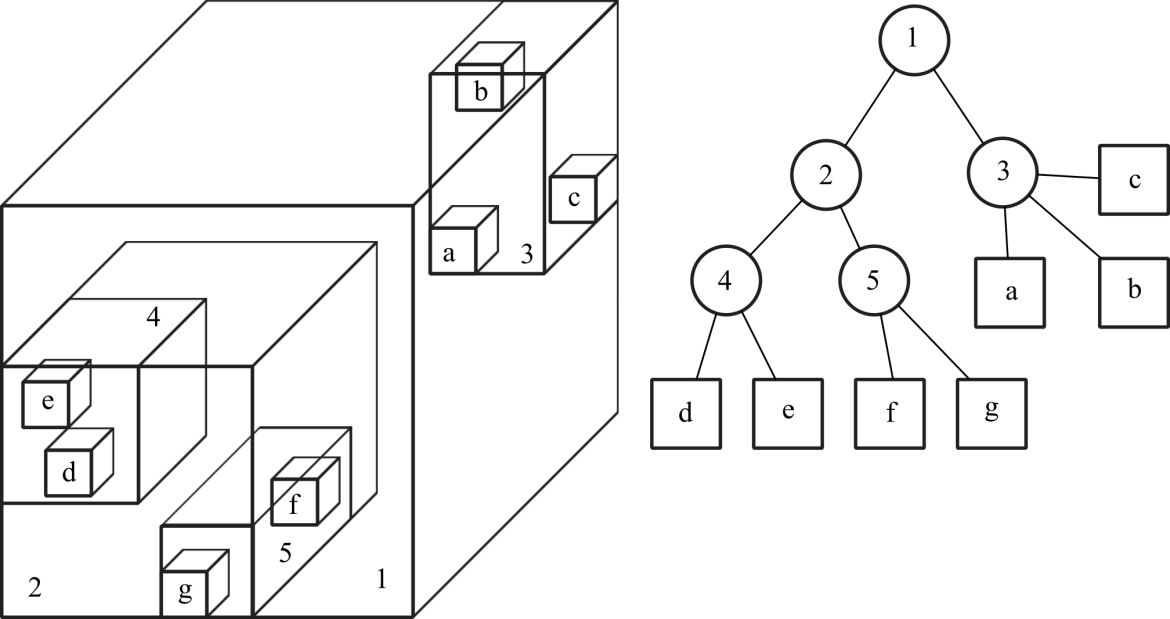
\includegraphics[width=0.6\linewidth]{Synopsis/images/bvh.png}
    \caption{Иерархия граничных объемов}
    \label{fig:bvh}
\end{figure}

Древовидная структура в случае удачного построения дерева позволяет
получить логарифмическую сложность. Худший случай представляет собой
такую ситуацию, при которой все примитивы сцены оказались в одном листе
древовидной структуры.
\[O\left( \log N \right) - \text{в среднем};O\left( n \right) - \text{в худшем случае.}\]


Форма непосредственно граничного объёма может быть различной:

\begin{itemize}
    \item
    сфера;
    \item
    AABB (Axis Aligned Bounding Box) -- прямоугольный параллелепипед вдоль
    осей координат;
    \item
    k-DOP (Discrete Oriented Polytope) -- дискретно-ориентированный
    многогранник.
    \item
    SSV (Swept Sphere Volume) -- объем покрывающих сфер;
    \item
    OBB (Oriented Bounding Box) -- прямоугольный параллелепипед
    ориентированный вдоль содержимого;
    \item
    сферическая оболочка;
    \item
    выпуклая оболочка.
\end{itemize}

Примеры форм граничного объема приведены на рисунке~\ref{fig:bvh-shapes}.

\begin{figure}[h]
    \centering
    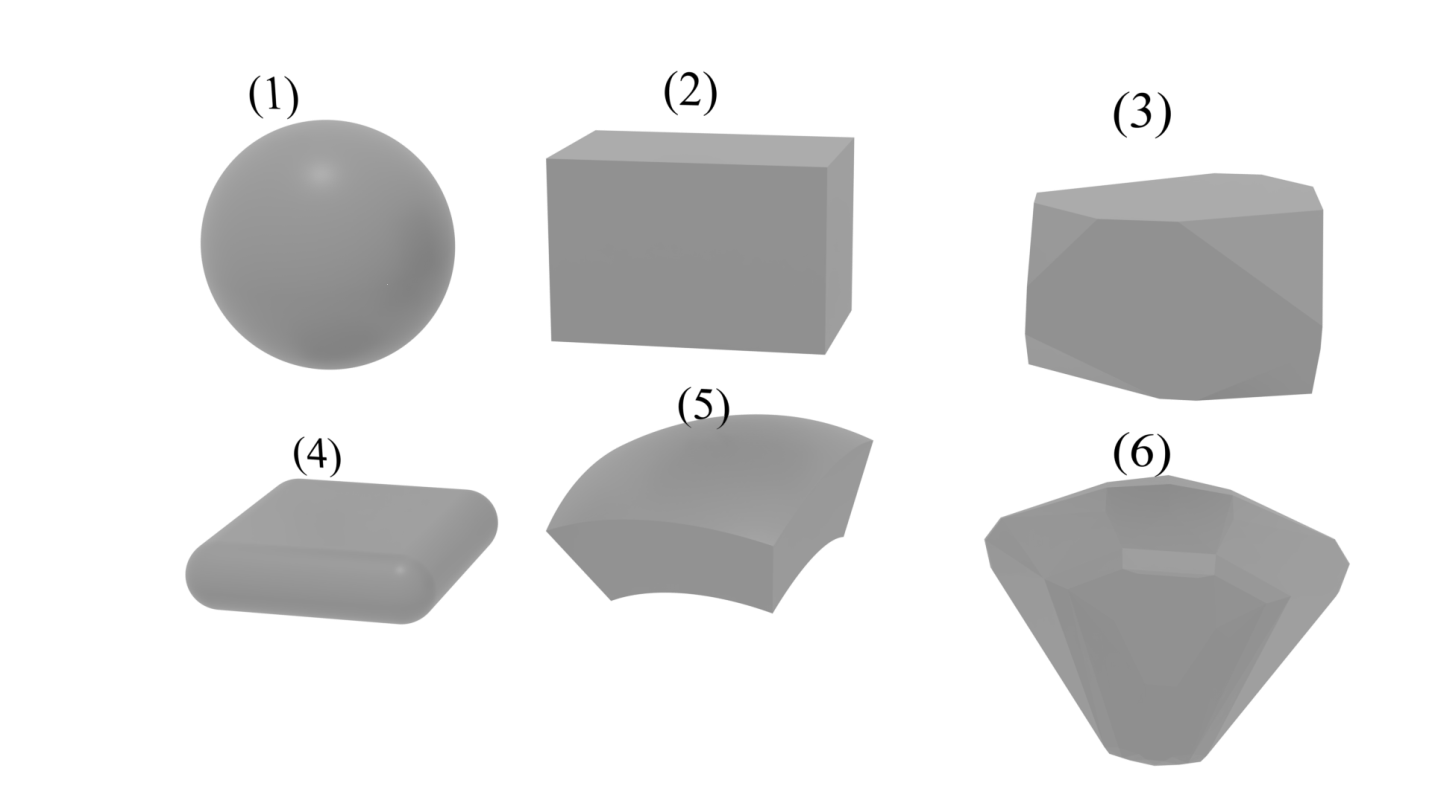
\includegraphics[width=0.7\linewidth]{Synopsis/images/bounding_volumes.png}
    \caption{Примеры форм граничного объема: (1) -- сфера; (2) --
        AABB; (3) -- 14-DOP; (4) -- SSV; (5) -- сферическая оболочка; (6) --
        выпуклая оболочка.}
    \label{fig:bvh-shapes}
\end{figure}

Различные варианты граничного объема представляют собой компромисс между
простотой операций построения и проверки попаданий и точностью
аппроксимации геометрии. Если граничный объем удачно аппроксимирует
объекты на сцене, то в процессе рейтрейсинга будет меньше случайных
попаданий в граничный объем, который находится на пути распространения
луча, однако не имеет ни одного вложенного элемента геометрии мешающего
пути луча.

В \textbf{подразделе 2.2} описана модель расчёта рассеянного поля в рамках физической
теории дифракции.
В частности полное поле складывается из полей падающей и рассеянной волны

\[ \mathbf{E}=\mathbf{E_{inc}} + \mathbf{E_{sca}}  \]
\[ \mathbf{H}=\mathbf{H_{inc}} + \mathbf{H_{sca}}  \]
Полное поле в начале координат описывается величинами $ \mathbf{E_0}$ и $\mathbf{H_0}$.
Положение точки на поверхности пластины (рис.~\ref{fig:facet_po}) задается радиус-вектором
$\mathbf{r}$. Единичный вектор $\hat{\mathbf{r}}_\mathbf{inc}$ определяет направление
рассеянной волны.
\begin{figure}[h]
    \center{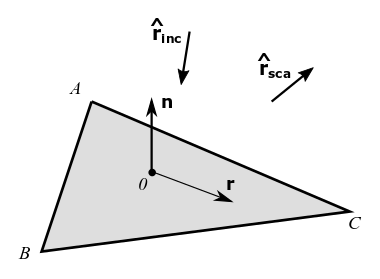
\includegraphics[width=0.40\linewidth]{Synopsis/images/facet_po.png}}
    \caption{Наклонное падение плоской волны полигональный фацет} \label{fig:facet_po}
\end{figure}

Подстановка в интеграл Стрэттона-Чу для дальней зоны дает
\[\mathbf{E_{sca}} = \frac{ik}{4\pi}\frac{e^{ikR}}{R}\int \limits_S \left[ \hat{\mathbf{r}}_{\mathbf{s}}\times (\mathbf{n} \times \mathbf{E}) + Z_0  \cdot \hat{\mathbf{r}}_\mathbf{s} \times \left( \hat{\mathbf{r}}_\mathbf{s} \times (\mathbf{n} \times \mathbf{H}) \right) \right] e^{-ik\hat{\mathbf{r}}_\mathbf{s} \mathbf{r}} \,dS  \]
В случае падения плоской волны поле в любой точке пластины можно выразить через значение поля в начале координат \autocite{knott2004radar}.
\begin{equation}
    \label{eq:FacetPOField}
    \mathbf{E_{sca}} = \frac{ik}{4\pi}\frac{e^{ikR}}{R}\left[ \hat{\mathbf{r}}_{\mathbf{s}}\times (\mathbf{n} \times \mathbf{E_0}) + Z_0  \cdot \hat{\mathbf{r}}_\mathbf{s} \times \left( \hat{\mathbf{r}}_\mathbf{s} \times (\mathbf{n} \times \mathbf{H_0}) \right) \right]\int \limits_S  e^{ik(\hat{\mathbf{r}}_\mathbf{inc}-\hat{\mathbf{r}}_\mathbf{s}) \mathbf{r}} \,dS
\end{equation}

Согласно теореме Стокса поверхностный интеграл заменяется контурным
\begin{equation}
    \label{eq:StokesTheorem}
    \int \limits_S ( \nabla \times \mathbf{A}) \mathbf{n}dS=\oint \limits_L \mathbf{Adl}
\end{equation}

В свою очередь контурный интеграл ломаному контуру сводится к сумме вкладов от каждого отрезка контура.

\begin{equation}
    \label{eq:Finite_difference}
    \oint \limits_L \mathbf{Adl} = L_{AB} + L_{BC} + L_{CA}
\end{equation}
Таким образом ресурсоёмкое вычисление поверхностного интеграла вырождается в эффективную сумму конечных разностей.



В \textbf{подразделе 2.3} предложена оригинальная модель расчёта рассеянного поля от
больш\'их площадных объектов, таких как различные типы земных покровов.

В интересных для практики случаях получение строгого решения задачи отражение от
шероховатой поверхности наталкивается на серьезные математические трудности. Это связано
со сложностью рельефа поверхности с произвольными радиусами кривизны ее участков, кроме
того, поверхность может быть неоднородной. Вследствие этого к определению характеристик
отражения от поверхностей с произвольной шероховатостью подходят следующим образом:
экспериментальным путем находят характеристики отражения при каких-то определенных
условиях (при нескольких углах визирования, длинах волн и т.п.), после чего синтезируют
модель поверхности. Структура модели подбирается таким образом, чтобы, с одной стороны,
расчет отраженного от нее поля был сравнительно прост, а с другой стороны, рассчитанные
характеристики были близки к характеристикам, полученным экспериментально.

Мощность отраженного сигнала на входе приемника РЛС зависит от целого ряда факторов и,
прежде всего, от отражающих свойств поверхности, характеризуемой эффективной площадью
рассеяния (ЭПР).

При углах зондирования, близких к вертикали, для большинства поверхностей отражение будет
близким к зеркальному, и будет наблюдаться наибольшие значения УЭПР. При углах
зондирования, близких к горизонтали, отражение будет очень малым. При промежуточных
значениях угла скольжения УЭПР, выраженная в дБ изменяется с ростом угла скольжения по
закону, близкому к линейному.

Для расчёта УЭПР была расширена полуэмпирическая модель, авторами которой являются Y.~Oh, K.~Scarabandi и T.~Ulaby\autocite{backscattering-soil}.
Была разработана база данных, собранная из научных источников, которая содержит
характеристики рассеяния однородных покровов Земли.

Для моделирования работы РЛС с заданной разрешающей способностью по азимуту и наклонной
дальности поверхность объекта должна быть представлена набором отражающих участков
(фацетов) одинаковой площади, равномерно распределенных по поверхности. При этом размеры
фацетов должны быть меньше параметров разрешающей способности РЛС.

При моделировании больших карт для уменьшения объёма памяти, занимаемой трёхмерной моделью
местности возникает необходимость менее детального представления природного ландшафта с
медленно меняющимися перепадами высот, такого как поле, дорога, водная поверхность и т.д.,
чем требуемое разрешение радиолокационного изображения. При этом при моделировании
возникает необходимость разбиения таких фацетов на более мелкие фацеты с заданной средней
площадью. При этом шероховатость поверхности модерируется с помощью наложения на
координаты центра фацета координатного шума с заданными параметрами.

Для решения заявленной проблемы разработан алгоритм заполнения треугольника точками с
равномерным распределением.
Данный алгоритм основан на формировании равномерной координатной сетки внутри треугольника
и размещении в узлах координатной сетки точек с последующим добавлением к координатам точек координатного шума.

В подразделе 2.4 приведены характеристики нескольких типов материалов в рамках предлагаемой модели отражений и
показаны их статистические оценки, соответствующие ожидаемым.


\underline{\textbf{Третья глава}} посвящена описанию программного комплекса.
В \textbf{подразделе 3.1} показана общая архитектура программного комплекса, описаны его
компоненты и показан пример задания геологической модели с помощью данного программного
комплекса. В \textbf{подразделе 3.2} описаны основные проблемы реализации программного
комплекса, возникающие на уровне требуемых вычислительных ресурсов и объёмов
оперативной памяти для хранения данных алгоритма. \textbf{Подраздел 3.3} содержит описание
реализации компоненты программного комплекса \textit{Источник-Граница}, которая вычисляет
волновое поле, распространяющееся от источника на границу модели, и представляет его в
векторной форме. \textbf{Подраздел 3.4} содержит описание реализации компоненты программного
комплекса \textit{Граница-Граница}, которая вычисляет рассеянное поле, распространяющееся от
предыдущей границы слоя на следующую в соответствии с заданным волновым кодом.
\textbf{Подраздел 3.5} содержит описание реализации компоненты программного комплекса \textit{Подлежащая
поверхность}, которая вычисляет волновое поле, распространяющееся от границы слоя в
приёмники. В \textbf{подразделе 3.6} рассмотрена реализация компоненты программного комплекса
\textit{Матрица Распространения}, которая представляет собой перемножение набора элементарных
матриц распространения крупных размерностей на набор векторов для дискретных частот.
Каждая матрица из набора заполняется по формулам. Процедура заполнения матриц
была оптимизирована, процедура перемножения матриц на векторы – адаптирована для параллельных архитектур.
В \textbf{подразделе 3.7} описаны сторонние программные средства, которые были использованы в
рамках реализации программного комплекса.




В \underline{\textbf{четвертой главе}} приведено описание вычислительных экспериментов и верификации

В \textbf{подразделе 4.1} проведена верификация результатов моделирования импедансных объектов
в рамках программной реализации предлагаемой модели и алгоритмов.
Рассматриваемый подход сравнивается решениями других алгоритмов и моделей,
среди которых:
\begin{description}
    \item[Expected] точное аналитическое решение;
    \item[IE] метод интегральных уравнений;
    \item[SBR] комбинация приближенных методов в пакете программного обеспечения Ansys HFSS;
    \item[Our] рассматриваемая в диссертации модель.
\end{description}
На рисунке \ref{fig:spherefront} представлена полигональная модель сферы, а на рисунках
\ref{fig:sphere} – \ref{fig:sphere1m} представлены результаты расчета ЭПР сферы точными и приближенными методами.

\begin{figure}[h]
    \centering
    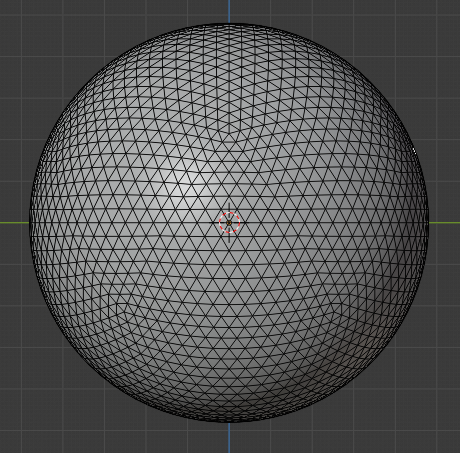
\includegraphics[width=0.3\linewidth]{Synopsis/images/sphere_front}
    \caption{Полигональная модель сферы}
    \label{fig:spherefront}
\end{figure}


\begin{figure}[h]
    \centering
    \begin{minipage}{0.49\textwidth}
        \centering
        \begin{tikzpicture}
            \begin{axis}
                [
                RCS Plot,
                restrict x to domain = 0:90,
                title={1 ГГц},
                xlabel={град},
                ylabel={дБм$^2$},
                ytick distance=1,
                legend pos = north east,
                ]
                \addplot table [x expr=\thisrowno{0}, y index=1] {Synopsis/data/sphere.csv};
                \addlegendentry{Our};
                \addplot+[domain=0:90] {10 * log10(0.0264)};
                \addlegendentry{Expected};
            \end{axis}
        \end{tikzpicture}
        \caption{Сфера $R=0,048$ м}
        \label{fig:sphere}
    \end{minipage}
    \hfill
    \begin{minipage}{0.49\textwidth}
        \centering
        \begin{tikzpicture}
            \begin{axis}
                [
                RCS Plot,
                restrict x to domain = 0:90,
                title={1 ГГц},
                xlabel={град},
                ylabel={дБм$^2$},
                ytick distance=1,
                legend pos = north east,
                ]
                \addplot table [x expr=\thisrowno{0}, y index=1] {Synopsis/data/sphere1m.csv};
                \addlegendentry{Our};
                \addplot+[domain=0:90] {10 * log10(3.2787698576191344)};
                \addlegendentry{Expected};
            \end{axis}
        \end{tikzpicture}
       	\caption{Сфера $R=1$ м}
        \label{fig:sphere1m}
    \end{minipage}
\end{figure}


\begin{figure}[h]
    \centering
    \noindent
    \begin{tikzpicture}
        \begin{loglogaxis}
            [
            RCS Plot,
            title={Сфера 1 м},
            height=0.4\textwidth,
            xlabel={ГГц},
            ylabel={ЭПР, м$^2$},
            ymin=0.01,
            legend pos = south east
            ]
            \addplot table {Synopsis/data/third-party/output2.dat};
            \addlegendentry{Exact};
            \addplot table {Synopsis/data/third-party/output.dat};
            \addlegendentry{SBR};
            \addplot+[mark=+, loosely dashed, semithick] table [x index=0, y index=1]{Synopsis/data/sphere1mfreq.csv};
            \addlegendentry{Our};
        \end{loglogaxis}
    \end{tikzpicture}
    \caption{Сходимость приближенных методов от соотношения размера объекта к длине волны}
    \label{fig:sphere1mfreq}
\end{figure}

Рисунки \ref{fig:sphere} и \ref{fig:sphere1m} показывают существенные отличия между
результатами моделирования и аналитическим решением для задачи расчёта ЭПР сферы.
На рисунке~\ref{fig:sphere1mfreq} показано, что для случая, когда геометрические размеры
объекта соизмеримы с длиной волны
физическая теория дифракции имеет серьёзные расхождения по сравнению с аналитическим
решением.

Для сферы значительное расхождение между точным решением и решением, полученном в
приближении физической оптики наблюдается в случае, когда радиус сферы сравним с длиной
волны. Это происходит потому, что на искривлённых поверхностях распределение
поверхностного тока значительно отличается от равномерной части тока, используемой в
приближении физической оптики. По мере увеличения частоты падающего излучения разница
между приближенным и точным решением уменьшается. Оба решения в коротковолновом пределе
стремятся к значению ЭПР обратного рассеяния, равному $\pi R^2$ , что также совпадает и с
решением, которое даёт геометрическая оптика.


На рисунке \ref{fig:ogive} представлена полигональная модель оживального тела, а на
рисунках \ref{fig:ogiveVV} – \ref{fig:ogiveHH} представлены результаты расчета ЭПР
оживального тела точными и приближенными методами.

\begin{figure}
    \centering
    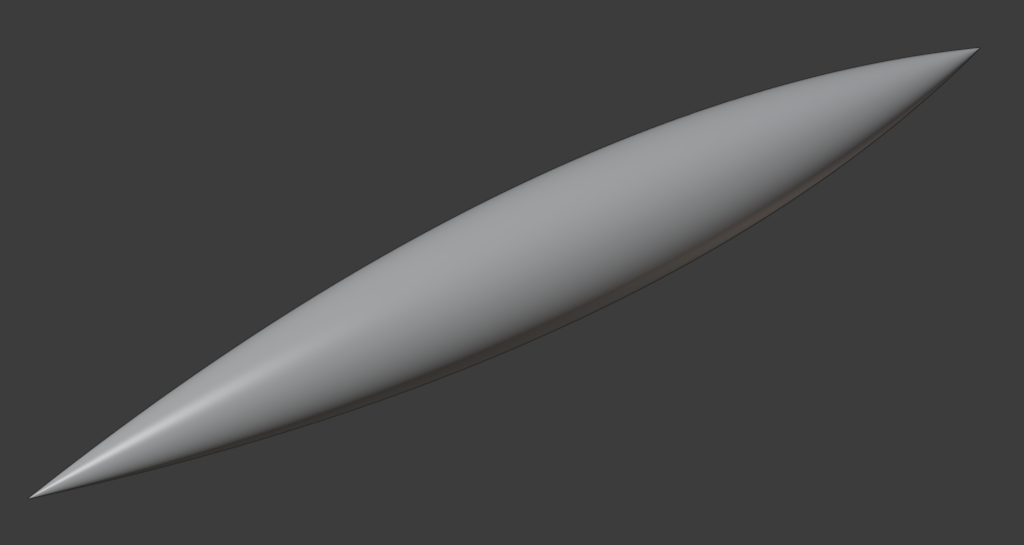
\includegraphics[width=0.5\linewidth]{Synopsis/images/Ogive}
    \caption{Полигональная модель оживального тела}
    \label{fig:ogive}
\end{figure}

\begin{figure}[h]
    \centering
    \begin{minipage}{0.49\textwidth}
        \centering
        \begin{tikzpicture}
            \begin{axis}
                [
                RCS Plot,
                restrict x to domain = 0:90,
                title={10 ГГц, VV},
                xlabel={град},
                ylabel={дБм$^2$},
                legend pos = south east,
                ]
                \addplot table [skip first n=7, x index=0, y expr = 10 * log10(\thisrowno{1})] {Synopsis/data/third-party/RCS Large Ogive Phi.txt};
                \addlegendentry{IE};
                \addplot table [skip first n=7, x index=0, y expr = 10 * log10(\thisrowno{1})] {Synopsis/data/third-party/RCS Large Ogive Phi SBR2.txt};
                \addlegendentry{SBR};
                \addplot table [x expr=\thisrowno{0}-90, y index=1] {Synopsis/data/ogive.csv};
                \addlegendentry{Our};
            \end{axis}
        \end{tikzpicture}
        \caption{Оживало $l=39 \lambda$, $\alpha = 15^\circ$}
        \label{fig:ogiveVV}
    \end{minipage}
    \hfill
    \begin{minipage}{0.49\textwidth}
        \centering
        \begin{tikzpicture}
            \begin{axis}
                [
                RCS Plot,
                restrict x to domain = 0:90,
                title={10 ГГц, HH},
                xlabel={град},
                ylabel={дБм$^2$},
                legend pos = south east,
                ]
                \addplot table [skip first n=7, x index=0, y expr = 10 * log10(\thisrowno{1})] {Synopsis/data/third-party/RCS Large Ogive Theta.txt};
                \addlegendentry{IE};
                \addplot table [skip first n=7, x index=0, y expr = 10 * log10(\thisrowno{1})] {Synopsis/data/third-party/RCS Large Ogive Theta SBR2.txt};
                \addlegendentry{SBR};
                \addplot table [x expr=\thisrowno{0}-90, y index=4] {Synopsis/data/ogive.csv};
                \addlegendentry{Our};
            \end{axis}
        \end{tikzpicture}
        \caption{Оживало $l=39 \lambda$, $\alpha = 15^\circ$}
        \label{fig:ogiveHH}
    \end{minipage}
\end{figure}

Подобная сфере картина наблюдается и для оживального тела. Значительное расхождение
наблюдается при падении волны вдоль длинной стороны оживального тела.


\begin{figure}
    \centering
    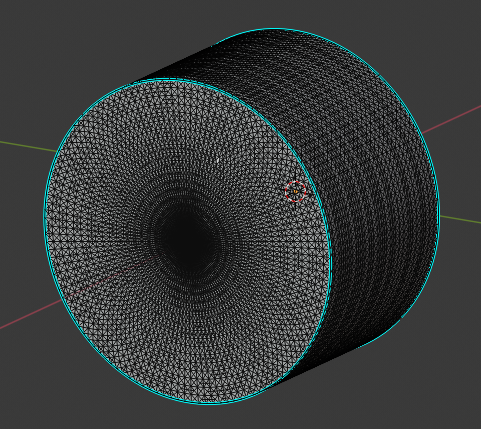
\includegraphics[width=0.3\linewidth]{Synopsis/images/cylinder_izo}
    \caption{Полигональная модель цилиндра}
    \label{fig:cylinderizo}
\end{figure}

\begin{figure}[h]
    \centering
    \begin{minipage}{0.49\textwidth}
        \centering
        \begin{tikzpicture}
            \begin{axis}
                [
                RCS Plot,
                title={10 ГГц, VV},
                xlabel={град},
                ylabel={дБм$^2$},
                legend pos = north east,
                ]
                \addplot table [skip first n=7, x index=0, y expr = 10 * log10(\thisrowno{1})] {Synopsis/data/third-party/RCS Cyl Phi IE.txt};
                \addlegendentry{IE};
                \addplot table [skip first n=7, x index=0, y expr = 10 * log10(\thisrowno{1})] {Synopsis/data/third-party/RCS Cyl Phi SBR.txt};
                \addlegendentry{SBR};
                \addplot table [x expr = \thisrowno{1} / pi * 180, y expr = 10 * log10(4 * pi * \thisrowno{3} * \thisrowno{3} + \thisrowno{4} * \thisrowno{4})] {Synopsis/data/cylinder.txt};
                \addlegendentry{Our};
            \end{axis}
        \end{tikzpicture}
        \caption{Цилиндр $R=4 \lambda$, $l=5 \lambda$}
        \label{fig:cylinderVV}
    \end{minipage}
    \hfill
    \begin{minipage}{0.49\textwidth}
        \centering
        \begin{tikzpicture}
            \begin{axis}
                [
                RCS Plot,
                title={10 ГГц, HH},
                xlabel={град},
                ylabel={дБм$^2$},
                legend pos = north east,
                ]
                \addplot table [skip first n=7, x index=0, y expr = 10 * log10(\thisrowno{1})] {Synopsis/data/third-party/RCS Cyl Theta IE.txt};
                \addlegendentry{IE};
                \addplot table [skip first n=7, x index=0, y expr = 10 * log10(\thisrowno{1})] {Synopsis/data/third-party/RCS Cyl Theta SBR.txt};
                \addlegendentry{SBR};
                \addplot table [x expr = \thisrowno{1} / pi * 180, y expr = 10 * log10(4 * pi * \thisrowno{9} * \thisrowno{9} + \thisrowno{10} * \thisrowno{10})] {Synopsis/data/cylinder.txt};
                \addlegendentry{Our};
            \end{axis}
        \end{tikzpicture}
        \caption{Цилиндр $R=4 \lambda$, $l=5 \lambda$}
        \label{fig:cylinderHH}
    \end{minipage}
\end{figure}

При расчёте ЭПР цилиндра наилучшее соотношение между точным и приближенным решениями
наблюдается в районе максимума ЭПР. Это также является особенностью приближенных методов
решения. Абсолютная погрешность определения рассеянного поля является приблизительно
одинаковой как в районах максимума амплитуды, так и в районах минимума. Это приводит к
большой относительной погрешности в районах минимума поля. Ситуация аналогична возрастанию
относительной погрешности при вычитании двух близких величин, определённых с погрешностью.


\begin{figure}
    \centering
    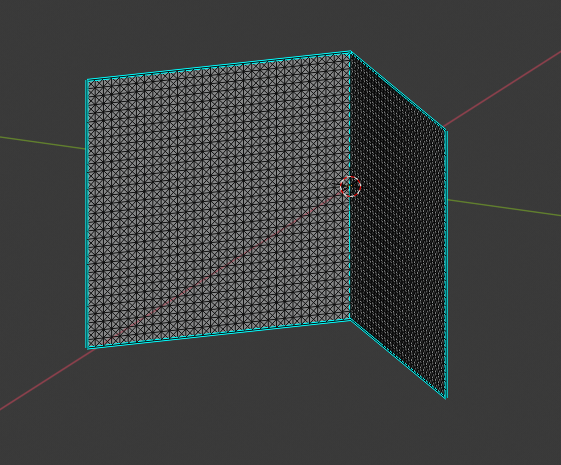
\includegraphics[width=0.4\linewidth]{Synopsis/images/ugol_izo}
    \caption{Полигональная модель двугранного уголкового отражателя}
    \label{fig:ugolizo}
\end{figure}


\begin{figure}[h]
    \centering
    \begin{minipage}{0.49\textwidth}
        \centering
        \begin{tikzpicture}
            \begin{axis}
                [
                RCS Plot,
                title={10 ГГц, VV},
                xlabel={град},
                ylabel={дБм$^2$},
                xtick distance=30,
                ymin=-40,
                legend pos = south west,
                restrict x to domain = 0:90,
                ]
                \addplot table [skip first n=7, x index=0, y expr = 10 * log10(\thisrowno{1})] {Synopsis/data/third-party/RCS Corner Phi IE.txt};
                \addlegendentry{IE};
                \addplot table [skip first n=7, x index=0, y expr = 10 * log10(\thisrowno{1})] {Synopsis/data/third-party/RCS Corner Phi SBR.txt};
                \addlegendentry{SBR};
                \addplot table [x expr = \thisrowno{2} / pi * 180, y expr = 10 * log10(4 * pi * (\thisrowno{9} * \thisrowno{9} + \thisrowno{10} * \thisrowno{10}))] {Synopsis/data/ugol.txt};
                \addlegendentry{Our};
            \end{axis}
        \end{tikzpicture}
        \caption{Двугранный уголковый отражатель $a=5,6 \lambda$}
        \label{fig:ugolVV}
    \end{minipage}
    \hfill
    \begin{minipage}{0.49\textwidth}
        \centering
        \begin{tikzpicture}
            \begin{axis}
                [
                RCS Plot,
                title={10 ГГц, HH},
                xlabel={град},
                ylabel={дБм$^2$},
                xtick distance=30,
                ymin=-40,
                legend pos = south west,
                restrict x to domain = 0:90,
                ]
                \addplot table [skip first n=7, x index=0, y expr = 10 * log10(\thisrowno{1})] {Synopsis/data/third-party/RCS Corner Theta IE.txt};
                \addlegendentry{IE};
                \addplot table [skip first n=7, x index=0, y expr = 10 * log10(\thisrowno{1})] {Synopsis/data/third-party/RCS Corner Theta SBR.txt};
                \addlegendentry{SBR};
                \addplot table [x expr = \thisrowno{2} / pi * 180, y expr = 10 * log10(4 * pi * (\thisrowno{3} * \thisrowno{3} + \thisrowno{4} * \thisrowno{4}))] {Synopsis/data/ugol.txt};
                \addlegendentry{Our};
            \end{axis}
        \end{tikzpicture}
        \caption{Двугранный уголковый отражатель $a=5,6 \lambda$}
        \label{fig:ugolHH}
    \end{minipage}
\end{figure}



Для двугранного уголкового отражателя хорошее совпадение наблюдается вблизи максимума ЭПР.
Для тех ракурсов, при которых одна из граней отражателя образует малый угол с направлением
падающей волны, наблюдается значительное расхождение между решением, полученным методом
интегральных уравнений и решением, полученным в приближении физической оптики.

При анализе систем типа открытого цилиндра результаты, полученные при использовании
приближенных методов, вряд ли следует считать достоверными, поскольку корректный анализ
поля при многократном отражении в системах типа резонаторов методами физической теории
дифракции затруднён и ведёт к большим погрешностям.

Физическая оптика, как часть физической теории дифракции исследует рассеяние волн на телах
сложной формы, размеры которых велики по сравнению с длиной волны. В рамках ФО рассеянное
телом поле рассматривается как излучение, которое создаётся поверхностными зарядами и
токами, возбуждаемыми падающей волной на поверхности тела.
Точное определение поверхностных токов является сложной задачей. Основные уравнения
физической оптики были получены на основе следующих предположений:
\begin{itemize}
    \item плотность тока, наводимого падающей волной в каждой точке освещённой области
    объекта равна плотности тока, который наводился бы на бесконечной плоскости,
    касательной к поверхности объекта в этой точке;
    \item в области тени плотность тока равна нулю.
\end{itemize}

Исходными данными для расчета являются значения поля падающих волн, рассчитанные в приближении геометрической оптики.

В физической теории дифракции предлагается учитывать более тонкие эффекты, связанные с
особенностями поля возле ребер и кромок и с попаданием токов на затененную часть гладкой
поверхности за счет волн соскальзывания.
Наряду с токами, возбуждаемыми на поверхности тела по законам геометрической оптики
(равномерные токи в терминологии физической теории дифракции) рассматриваются
дополнительные токи, возникающие вблизи ребер и краев, имеющие характер краевых волн и
быстро ослабевающие при удалении от ребра или края. В ситуации, когда величина объекта соизмерима с длинной волны, грани на полигональной поверхности находятся слишком близко по отношению друг к другу и в таком случае нельзя предполагать отсутствие влияния тока одного ребра на другое.

В \textbf{подразделе 4.2} проведена верификация результатов моделирования подстилающей поверхности.

\begin{figure}[h]
    \centering
    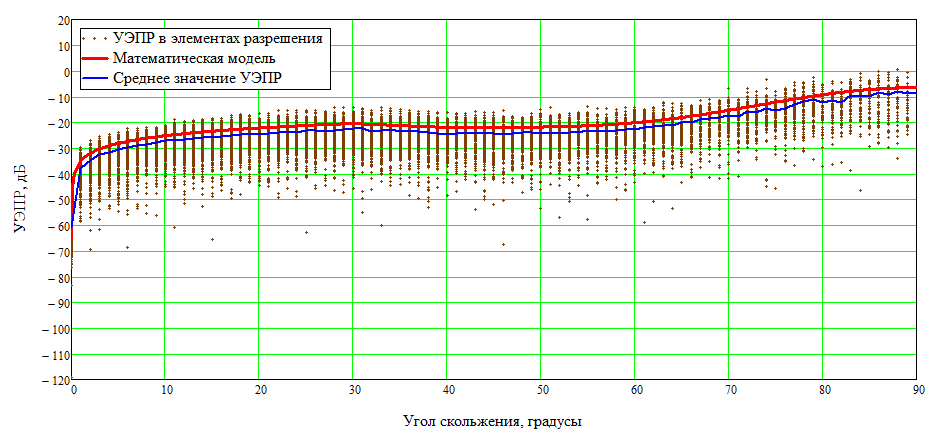
\includegraphics[width=0.9\linewidth]{Synopsis/images/surface_grass}
    \caption{Зависимость УЭПР травы при изменении угла скольжения}
    \label{fig:surfacegrass}
\end{figure}
\begin{figure}[h]
    \centering
    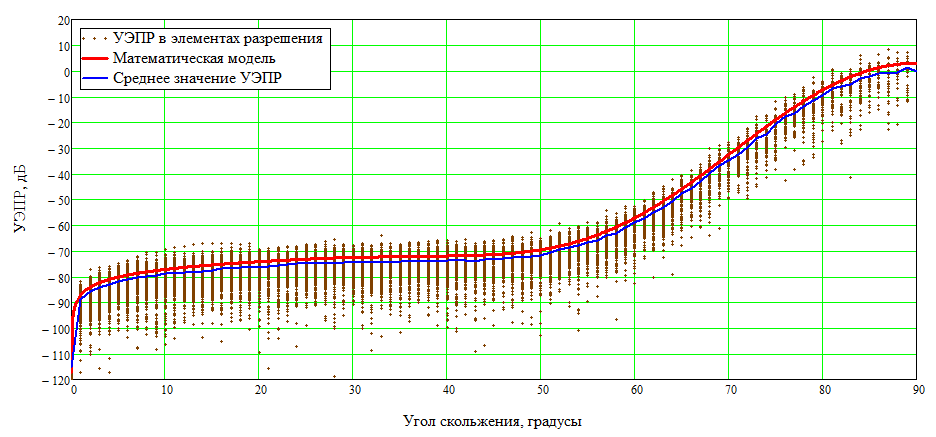
\includegraphics[width=0.9\linewidth]{Synopsis/images/surface_water}
    \caption{Зависимость УЭПР поверхности спокойной воды при изменении угла скольжения}
    \label{fig:surfacewater}
\end{figure}

Результат работы разработанного алгоритма позволяет получить статистические характеристики УЭПР с распределением вероятности соответствующим ожидаемому распределению Релея. %????

\begin{figure}
    \centering
    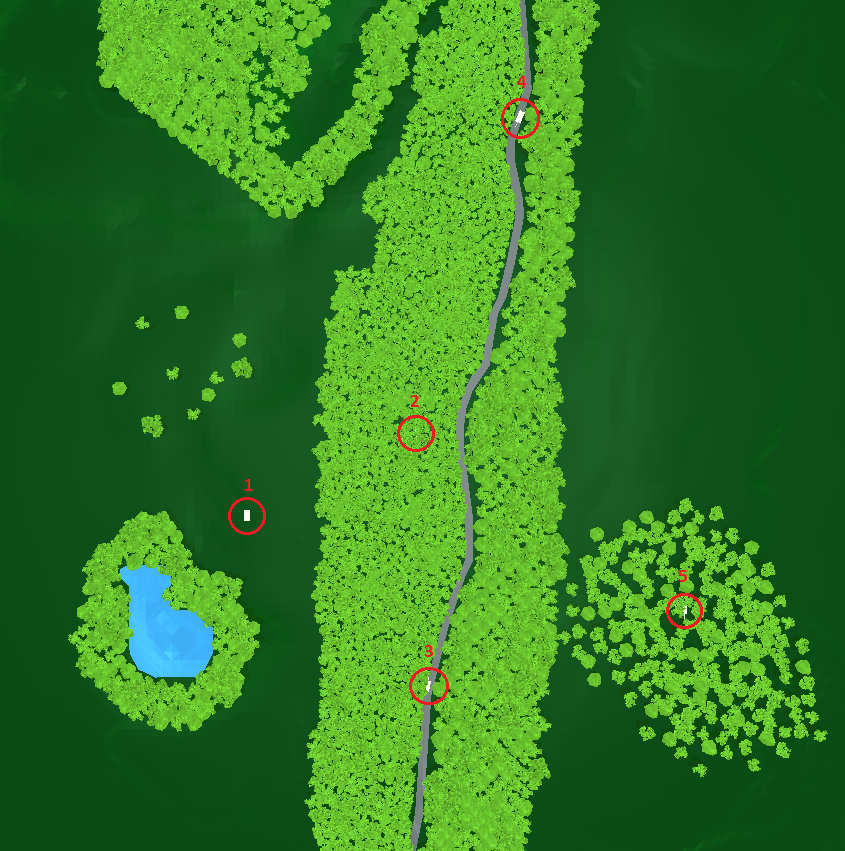
\includegraphics[width=0.7\linewidth]{Synopsis/images/top}
    \caption{Пример радиолокационной сцены}
    \label{fig:top}
\end{figure}

В \textbf{подразделе 4.3} проведена верификация непосредственно радиолокационных изображений полученных на разработанном программном комплексе. Рассмотрены задачи выбора оптимального частотного диапазона, для обнаружения лёгкой и тяжёлой техники.
На рисунке \ref{fig:top} представлена полигональная модель сцены, на поверхности которой размещены как различные покровы Земли, так и разные варианты техники.


\begin{figure}
    \centering
    \includegraphics[width=0.7\linewidth]{Synopsis/images/forest_X_RD}
    \caption{Результат работы программного комплекса}
    \label{fig:forestxrd}
\end{figure}

На рисунке \ref{fig:forestxrd} представлен результат работы программного комплекса, который с одной стороны качественно имеет эффекты присущие радиоэлектронным изображениям, такие как спекл-шум, радиотень, радиопрозрачность и паразитные боковые лепестки. С другой стороны количественно отслеживаются статистические характеристики спекл шума, перерасчитывается энергетика и удельные ЭПР поверхностей. Решаются задачи радиокоррекции.

\FloatBarrier
\pdfbookmark{Заключение}{conclusion}                                  % Закладка pdf
В \underline{\textbf{заключении}} приведены основные результаты работы, которые заключаются в следующем:
\input{common/concl}

\pdfbookmark{Литература}{bibliography}                                % Закладка pdf
%При использовании пакета \verb!biblatex! список публикаций автора по теме
%диссертации формируется в разделе <<\publications>>\ файла
%\verb!common/characteristic.tex!  при помощи команды \verb!\nocite!

\ifdefmacro{\microtypesetup}{\microtypesetup{protrusion=false}}{} % не рекомендуется применять пакет микротипографики к автоматически генерируемому списку литературы
\urlstyle{rm}                               % ссылки URL обычным шрифтом
\ifnumequal{\value{bibliosel}}{0}{% Встроенная реализация с загрузкой файла через движок bibtex8
    \renewcommand{\bibname}{\large \bibtitleauthor}
    \nocite{*}
    \insertbiblioauthor           % Подключаем Bib-базы
    %\insertbiblioexternal   % !!! bibtex не умеет работать с несколькими библиографиями !!!
}{% Реализация пакетом biblatex через движок biber
    % Цитирования.
    %  * Порядок перечисления определяет порядок в библиографии (только внутри подраздела, если `\insertbiblioauthorgrouped`).
    %  * Если не соблюдать порядок "как для \printbibliography", нумерация в `\insertbiblioauthor` будет кривой.
    %  * Если цитировать каждый источник отдельной командой --- найти некоторые ошибки будет проще.
    %
    %% authorvak
%    \nocite{vakbib1}%
%    \nocite{vakbib2}%
    %
    %% authorwos
%    \nocite{wosbib1}%
    %
    %% authorscopus
    \nocite{Leukhin2020multiphase}
    \nocite{Leukhin2020autofocusing}
    \nocite{Leukhin2020binary}
    \nocite{Leukhin2019}
    \nocite{Leukhin2019xp}
    \nocite{Leukhin2018}
    \nocite{Rozhentsov20181068}
    \nocite{Voronin20181}
    \nocite{Leukhin201825}
    \nocite{Karasev2018336}
    \nocite{Leukhin2018330}
    %\nocite{Leukhin2017}
    %
    %% authorpathent
%    \nocite{patbib1}%
    %
    %% authorprogram
%    \nocite{progbib1}%
    %
    %% authorconf
%    \nocite{confbib1}%
%    \nocite{confbib2}%
    %
    %% authorother
%    \nocite{bib1}%
%    \nocite{bib2}%

    \ifnumgreater{\value{usefootcite}}{0}{
        \begin{refcontext}[labelprefix={}]
            \ifnum \value{bibgrouped}>0
                \insertbiblioauthorgrouped    % Вывод всех работ автора, сгруппированных по источникам
            \else
                \insertbiblioauthor      % Вывод всех работ автора
            \fi
        \end{refcontext}
    }{
        \ifnum \totvalue{citeexternal}>0
            \begin{refcontext}[labelprefix=A]
                \ifnum \value{bibgrouped}>0
                    \insertbiblioauthorgrouped    % Вывод всех работ автора, сгруппированных по источникам
                \else
                    \insertbiblioauthor      % Вывод всех работ автора
                \fi
            \end{refcontext}
        \else
            \ifnum \value{bibgrouped}>0
                \insertbiblioauthorgrouped    % Вывод всех работ автора, сгруппированных по источникам
            \else
                \insertbiblioauthor      % Вывод всех работ автора
            \fi
        \fi
        %  \insertbiblioauthorimportant  % Вывод наиболее значимых работ автора (определяется в файле characteristic во второй section)
        \begin{refcontext}[labelprefix={}]
            \insertbiblioexternal            % Вывод списка литературы, на которую ссылались в тексте автореферата
        \end{refcontext}
        % Невидимый библиографический список для подсчёта количества внешних публикаций
        % Используется, чтобы убрать приставку "А" у работ автора, если в автореферате нет
        % цитирований внешних источников.
        \printbibliography[heading=nobibheading, section=0, env=countexternal, keyword=biblioexternal, resetnumbers=true]%
    }
}
\ifdefmacro{\microtypesetup}{\microtypesetup{protrusion=true}}{}
\urlstyle{tt}                               % возвращаем установки шрифта ссылок URL
